\documentclass[11pt]{article}
\usepackage[margin=0.85in]{geometry}
\usepackage{fontspec}
\setmainfont{Helvetica Neue}[
  UprightFont = * Medium,
  BoldFont    = * Bold,
  ItalicFont  = * Medium Italic,
]
\setmonofont{Menlo}[Scale=0.92]
\usepackage{xcolor}
\usepackage{graphicx}
\usepackage{booktabs}
\usepackage{amsmath, amssymb}
\usepackage{enumitem}
\setlist{nosep, leftmargin=1.2em, itemsep=2pt}
\usepackage{titlesec}
\usepackage[colorlinks=true,urlcolor=blue!50!black,linkcolor=black,citecolor=black]{hyperref}

\definecolor{accent}{HTML}{B31B1B}

\setlength{\parindent}{0pt}
\setlength{\parskip}{3pt}
\titlespacing*{\section}{0pt}{7pt}{3pt}

\title{\vspace{-2em}\textbf{Reproducing LoRA on RoBERTa-base}\\
       \large CS 4782 Final Project Summary}
\author{Lucas He, Partner \\
        \small Cornell University, Spring 2026}
\date{\vspace{-1em}}

\begin{document}
\maketitle
\vspace{-1.7em}

\section*{1. Goal}

LoRA freezes pretrained weights and learns a low-rank update
$\Delta W = BA$ on selected matrices, aiming to match full fine-tuning with
far fewer trainable parameters. We reproduce Hu et al.'s RoBERTa-base GLUE
result and test whether the low intrinsic-rank claim holds on MRPC. We then
ask a further question: can LoRA absorb an attention-level architectural
change, Exclusive Self-Attention (XSA), when inserted only at fine-tuning time?

\section*{2. Setup}

We target the RoBERTa$_\text{base}$ + LoRA result on GLUE MRPC from Hu et
al. (2021), then rerun the rank ablation $r \in \{1,2,4,8\}$ on MRPC. As a
secondary task, we also run SST-2 at $r{=}8$. This slice tests both the
parameter-efficiency claim---LoRA gives most of full fine-tuning's benefit
with few trainable weights---and the intrinsic-rank claim---larger $r$ should
not matter much once the update has enough rank.

We implement LoRA directly by wrapping each attention \texttt{query} and
\texttt{value} projection in RoBERTa-base with a trainable low-rank update,
freezing the original linear weights and training only LoRA parameters plus
the classifier head. We train with AdamW, batch size 32, max length 128, seed
42, and linear warmup/decay. LoRA uses learning rate $5\!\times\!10^{-4}$;
full fine-tuning uses $2\!\times\!10^{-5}$. MRPC runs for 3 epochs, while
SST-2 runs for 2000 steps due to wall-clock budget. We also include a frozen
head-only baseline to verify that LoRA's gains come from low-rank adaptation
rather than the classifier alone.

\section*{3. Reproduction results}

On MRPC, full fine-tuning reaches 88.2\%, LoRA $r{=}8$ reaches 86.3\%, LoRA
$r{=}1$ reaches 86.0\%, and the head-only baseline reaches 68.4\%. Although
our LoRA result is below the paper's reported 87.5\%, the 18-point gap over
head-only confirms that the low-rank update, not just the new classifier, is
doing the adaptation.

\begin{center}
\small
\begin{tabular}{lrrrr}
\toprule
$r$ & 1 & 2 & 4 & 8 \\
Trainable params & 629K & 666K & 739K & 887K \\
MRPC accuracy & 0.860 & 0.858 & 0.865 & 0.863 \\
\bottomrule
\end{tabular}
\end{center}

The spread across ranks is only 0.7 points, within the noise expected on the
408-example MRPC validation set. This reproduces the qualitative finding that
increasing $r$ does not unlock much additional performance, suggesting that
the useful fine-tuning update has low intrinsic rank. On SST-2, LoRA $r{=}8$
reaches 93.1\% in roughly one epoch, compared with the paper's 95.1\% after a
full sweep. We therefore match the paper's main trend, though not its exact
absolute accuracy, likely because our runs are single-seed and lightly tuned.

\section*{4. Additional exploration: LoRA under Exclusive Self-Attention}

We also tested whether LoRA can absorb an attention-level architectural
change at fine-tuning time. Exclusive Self-Attention (XSA) projects each
head's attention output away from its own value vector,
$Y \leftarrow Y - (Y \cdot V_n)V_n$, with $V_n=V/\|V\|$, to reduce
self-similarity bias. Because XSA was proposed for from-scratch training, we
asked whether a pretrained RoBERTa-base model could tolerate the change when
only LoRA and the classifier head are trainable.

\begin{center}
\small
\begin{tabular}{lccccc}
\toprule
 & MRPC $r{=}1$ & $r{=}2$ & $r{=}4$ & $r{=}8$ & SST-2 $r{=}8$ \\
\midrule
Baseline LoRA & .860 & .858 & .865 & .863 & .931 \\
LoRA + XSA    & .848 & .853 & .855 & .850 & .922 \\
$\Delta$      & $-1.2$ & $-0.5$ & $-1.0$ & $-1.3$ & $-0.9$ \\
\bottomrule
\end{tabular}
\end{center}

\begin{center}
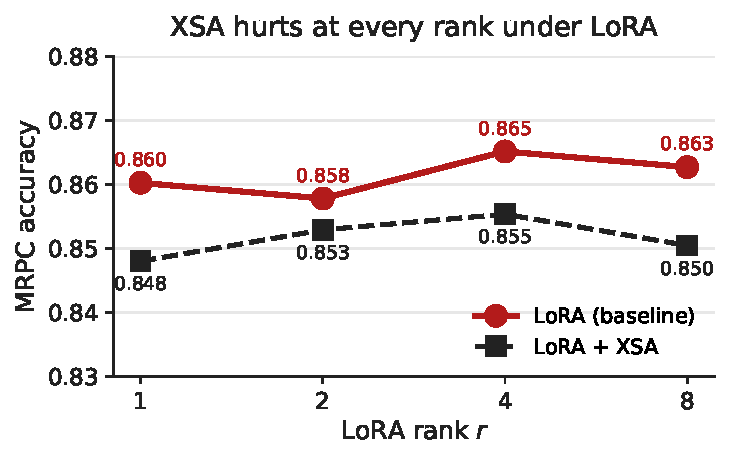
\includegraphics[width=0.62\linewidth]{../figures/xsa_comparison.pdf}
\end{center}

XSA consistently hurts by about one accuracy point in our single-seed runs.
The runs remain stable, so the issue is not optimization collapse; rather,
XSA changes the representation distribution in every attention layer after
pretraining. This suggests that XSA is not a drop-in fine-tuning-time
modification for standard pretrained RoBERTa under a small LoRA budget. A
natural follow-up is full fine-tuning with XSA to test whether the gap is due
to adaptation capacity rather than the XSA constraint itself.

\section*{5. Takeaways}

Our reproduction supports the qualitative LoRA claim: a tiny low-rank update
to $W_q$ and $W_v$ gives most of the benefit of full fine-tuning, while rank
has little effect on MRPC once $r \geq 1$. The main mismatch with the paper is
absolute accuracy, likely due to single-seed fixed-hyperparameter runs. The
XSA experiment is a useful negative result: LoRA trains stably under the
modified attention rule, but does not fully compensate for the layerwise
distribution shift introduced after pretraining.

{\small References: Hu et al. (2021), \emph{LoRA: Low-Rank Adaptation of
Large Language Models}; Liu et al. (2019), \emph{RoBERTa}; Wang et al. (2019),
\emph{GLUE}; Aghajanyan et al. (2020), \emph{Intrinsic Dimensionality Explains
the Effectiveness of Language Model Fine-Tuning}.}

\end{document}
